\documentclass{report}
\usepackage[margin=1in, paperwidth=8.5in, paperheight=11in]{geometry}
%Math packages%
\usepackage{amsmath}
\usepackage{amssymb}
%\usepackage{MnSymbol}
\usepackage{amsthm}
%Spacing%
\usepackage{setspace}
\onehalfspacing
%Lecture number%
\newcommand{\lectureNum}{21}
%Variables - Date and Course%
\newcommand{\curDate}{February 27, 2017}
\newcommand{\course}{MATH 239}
\newcommand{\instructor}{Luke Postle}
%Defining the example tag%
%\theoremstyle{definition}%
\newtheorem{ex}{Example}[section]
%Setting counter given the lecture number%
\setcounter{chapter}{\lectureNum{}}
%Package for drawing graphs%
\usepackage{tikz}
\usepackage{verbatim}
\usetikzlibrary{arrows}

\begin{document}
%Note title%
\begin{center}
\begin{Large}
\textsc{\course{} | Lecture \lectureNum{}}
\end{Large}
\end{center} 
\noindent \textit{Bartosz Antczak} \hfill
\textit{Instructor: \instructor{}} \hfill
\textit{\curDate{}}
\rule{\textwidth}{0.4pt}
%Actual Notes%
\subsubsection{Midterm Info}
The midterm will cover only graph theory | \textbf{up to Matching and Covers}. This means that there's \textit{no Konig's Theorem, Bipartite Matching Algorithm, or Hall's theorem.}\\
About half the exam is algorithmic (i.e., find an Eulerian circuit, find a particular colouring). The other half is proofs, some are easy (i.e., using Euler's formula) and others are more challenging.
\section{Intro to Enumerative Combinatorics}
One big topic in Combinatorics is graph theory (which was the first part of this course). Another big topic is counting, or \textit{enumerative combinatorics}. It involves counting discrete objects (e.g., a graph, binary strings, compositions).
\begin{ex}
Examples for counting graphs:
\end{ex}
\begin{itemize}
\item How many graphs are there on $n$ vertices?
\item How many trees are there on $n$ vertices?
\item How many matchings (or perfect matchings) of $K_n$ are there?\\
\textit{For instance, in $K_4$, there's \textbf{3} perfect matchings on labelled vertices:}
\begin{center}
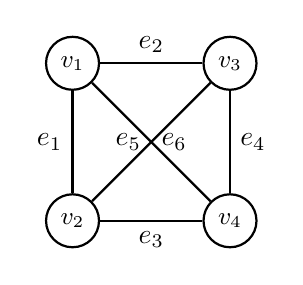
\begin{tikzpicture}[-,auto,node distance=2cm,
                    thick,main node/.style={circle,draw,font=\sffamily\small}]

  \node[main node] (1) {$v_1$};
  \node[main node] (2) [below of=1] {$v_2$};
  \node[main node] (3) [right of=1] {$v_3$};
  \node[main node] (4) [below of=3] {$v_4$};
  
  \path[every node/.style={font=\sffamily}]
    (1) edge  node [left] {$e_1$} (2)
    	edge node [above] {$e_2$} (3)
    	edge node [left]{$e_5$}(4)
    (2) edge node [right]{$e_6$}(3)
    (4) edge node [below] {$e_3$} (2)
    	edge  node [right] {$e_4$} (3);
\end{tikzpicture}
\end{center}
The matchings are $M_1 = \{e_1, e_4\}, M_2 = \{e_2, e_3\}, M_3 = \{e_5, e_6\}$.
\end{itemize}
\subsection{How to Count}
The basic operations for numbers are:
\begin{itemize}
\item Addition ($+$) [Plus its inverse, subtraction]
\item Multiplication ($\times$) [Plus its inverse, division]
\item Equality ($=$)
\end{itemize}
We can apply these operations on objects in sets
\begin{center}
\begin{tabular}{ c | c }
\textbf{Numbers} & \textbf{Sets} \\ \hline
$+$ & \textit{Disjoint Union} \\
$\times$ & \textit{Cartesian Product} \\
$=$ & \textit{Bijection}
\end{tabular}
\end{center}
\subsubsection{Disjoint Unison}
$B$ is the \textbf{disjoint union} of $A_1$ and $A_2$ if $B = A_1 \cup A_2$ and $A_1, A_2$ are disjoint (i.e., $A_1 \cap A_2 = \emptyset$. Denoted as $$B = A_1 \sqcup  A_2$$
We can also extend this definition to many sets, $B$ is the disjoint union of $A_1, A_2, \cdots, A_k$ if $B = A_1 \cup A_2 \cup \cdots A_k$ and $\forall i \neq j, A_i \cap A_j = \emptyset$. A proposition arises from this:
\begin{center}
\textit{If $B = A_1 \sqcup  A_2 \sqcup  \cdots A_k$, then $|B| = |A_1| + |A_2| + \cdots |A_k| = \displaystyle\sum_{i=1}^k |A_i|$}
\end{center}
\textbf{Remark:} if $B = A_1 \sqcup  A_2 \sqcup \cdots A_k$, then we say that $(A_1, A_2, \cdots, A_k)$ is a \textit{partition} of $B$.
\subsubsection{Cartesian Product}
$B$ is the \textbf{Cartesian product} of $A_1$ and $A_2$ is $B$ is the set of ordered pairs whose 1st elements are in $A_1$ and the 2nd element in $A_2$. This is denoted as
$$B = A_1 \times A_2 = \{(a_1, a_2) \,:\,a_1 \in A_1,\, a_2 \in A_2 \}$$
A common example of this is the plane of all real numbers, $\mathbb{R}^2 = \{(x,y) \, : \, x,y \in \mathbb{R}\}$. From this, a proposition arises:
\begin{center}
\textit{If $B = A_1 \times A_2 \times \cdots \times A_k$, then $|B| = |A_1| \cdots |A_2| \cdots |A_k| = \displaystyle\prod_{i=1}^k |A_i|$}
\end{center}
If the same set is used in the product, this is called a \textbf{Cartesian power}. For example, if $$B = A \times A \times \cdots_{k\mathrm{\,\,times}} \times A = A^k$$
A common example is $R^n$.
\subsubsection{Bijection}
A \textbf{bijection} from a set $A$ to a set $B$ is a 1-1 (i.e., one-to-one) mapping (or function) from $A$ to $B$. Let's consider a proposition:
\begin{center}
\textit{If there exists a bijection from A to B, then $|A| = |B|$}
\end{center}
\subsection{Binary Strings}
A \textbf{binary string} is a sequence of zeros and ones. Its length is the number of digits. Some examples include: $001, 1010, 00101, 1101, \cdots$.
\subsubsection{How many binary strings are there of length n?}
The answer is $2^n$. This works even when $n = 0$. This returns a value of 1, and this is correct. When $n=0$, we have only the empty string $\varepsilon$.\\There exists a formal proof showing that there are $2^n$ possible binary strings of length $n$. In short, it involves a bijection of $\{0,1\}^n$. More on this next lecture.
%END%
\end{document}